
\section{Method}

In this section, we will describe the methods used for face and emotion recognition. We also discuss the datasets and propose the methods we will use to make use of them. All of these methods are proposed with consideration that we need to achieve a minimum viable product for our robot. As this is a project oriented to produce a physical prototype, we have to consider that experimental results will have an impact when deciding the final implementation of the features and how much of a compromise between quality and performance we are willing to make. 


To achieve a MVP (Minimum Viable Product) and be worthy of a MSc project, we set our goals as the following:
\begin{itemize}
  \item Remove the need to use Google's Cloud API for all computer vision tasks, implementing local solutions.
  \item Implement new routines involving engaging computer vision algorithms like Style Transfer.
  \item The user should easily be able to obtain the style transferred files.
  \item The visual representation on the screen should be at least visually pleasing enough that users will want to keep it on as a background element.
  \item Make the robot completely autonomous: remove the need to offload computation to a 3rd party service or a local machine.
  \item Achieve a real-time representation of the robot's image processing.
\end{itemize}

\subsection{Face detection}

Previously, our pipeline for the robot required sending images to Google's Cloud Services (GCS) for emotion recognition. As we have removed GCS, this is no longer the case. To replace the previous face detection + emotion detection parts of the pipeline, we need to implement local methods face detection and emotion detection based off state of the art methods. Face detection allows the arm to follow a subject should it approach the limits of the camera's viewing angle. We propose using a Haar-Cascade classifier to detect faces. 

\subsection{Emotion recognition}
Detecting faces in the frame also serves to improve emotion detection, as described in Gunwan et al.\cite{haarcrop}, a neural network trained on cropped faces performs optimally on similiarly cropped images. We propose training a network on the FERPlus\cite{BarsoumICMI2016} dataset.


\subsection{FERPlus Dataset}

The FERPlus dataset, published by Barsoum et. al\cite{BarsoumICMI2016}, is an improvement over a the previous FER\cite{FER2013} dataset published for a \emph{Kaggle.com} research competition.

FER, prepared by Pierre-Luc Carrier and Aaron Courville. Each image measuring 48 pixels wide and high the dataset consists of ~28k images. The dataset annotations consist of numeric codes ranging from 0 to 6 for the emotion present in the image file: \emph{(0=Angry, 1=Disgust, 2=Fear, 3=Happy, 4=Sad, 5=Surprise, 6=Neutral).}
The FERPlus dataset improves the previous FER dataset by re-tagging the dataset manually\ref{fig:fervsferplus}. FERPlus adds more classes, bringing it up to 8 emotions total. Each image has been labeled by 10 independent "taggers" (humans), which means that each face image has a distribution of emotions.


\begin{figure}[h]
  \centering
  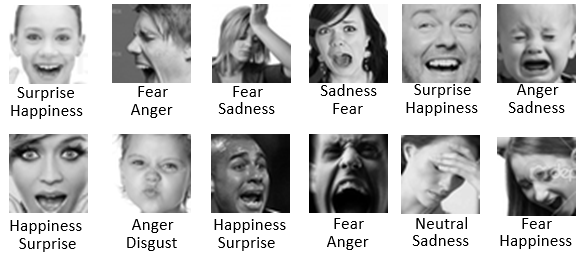
\includegraphics[width=10cm]{resources/fervsferplus.png}
  \caption{Comparison of FER and FERplus labels.}\label{fig:fervsferplus}
\end{figure}


While FERPlus authors used a custom VGG13 model for training, we propose using a recent VGG model (VGG19) for our implementation. 


\subsection{Style transfer method proposal}

Emotion detection will be used to change the context of the style transfer network, loosely adapting the target style transfer to a user's visible emotional status.


We propose a local implementation of a neural network capable of producing style transfer images as close to real-time on the Raspberry Pi 4's hardware as possible. The models can be pre-trained in a more powerful environment, but inference should run completely locally on the device, so no external connections or dependencies are needed in run-time. We propose experimenting with two different architectures: a recent model that requires more potent hardware but has better performance (results), and an older model that does not require high-end hardware, producing worse results, but potentially giving us faster results and allowing the robot to run inference locally. Thus, we propose adapting Karras' StyleGAN2 representing the "state of the art" method, and since we are already using VGG16 and VGG19 models for our emotion recognition, adapting the method proposed by Justin Johnson et. al on their \emph{"Perceptual Losses for Real-Time Style Transfer
and Super-Resolution"} \cite{Johnson2016Perceptual} publication representing the "old but fast" method to run on our hardware.
While StyleGAN2 was trained using the FFHQ dataset \cite{nvlabs_2019}, we propose using Microsoft's COCO 2014 training dataset\cite{DBLP:journals/corr/LinMBHPRDZ14} to train our style transfer models, as we are not using only face images on our style transfer. 

If one of these two methods is able to run locally while acheiving a good framerate, it should be strongly chosen for the final implementation, as it would complete our final two objectives for an MVP.



\subsection{COCO 2014 dataset}

Microsoft's COCO 2014 training dataset was released as part of a larger publication containing training, validation and test images. Totaling 328K images, it was the largest and most curated dataset at it's publication. The dataset contains 80 different classes and multiple captions per image. 